\documentclass[final, 12pt, aspectratio=169]{beamer}
\usepackage[utf8]{inputenc}
\usenavigationsymbolstemplate{\beamertemplatenavigationsymbolsempty}

\usepackage{graphicx}
\usepackage{tikz}
\usetikzlibrary{positioning}

\begin{document}
\begin{frame}
\center{
\Large{Genealogies of Sequential Monte Carlo Algorithms}\\[3pt]
\normalsize{Suzie Brown}\\[10pt]
\hrule
}

\vspace*{50pt}

\begin{columns}
\begin{column}{0.45\paperwidth}
\begin{center}
\resizebox{0.9\textwidth}{!}{%
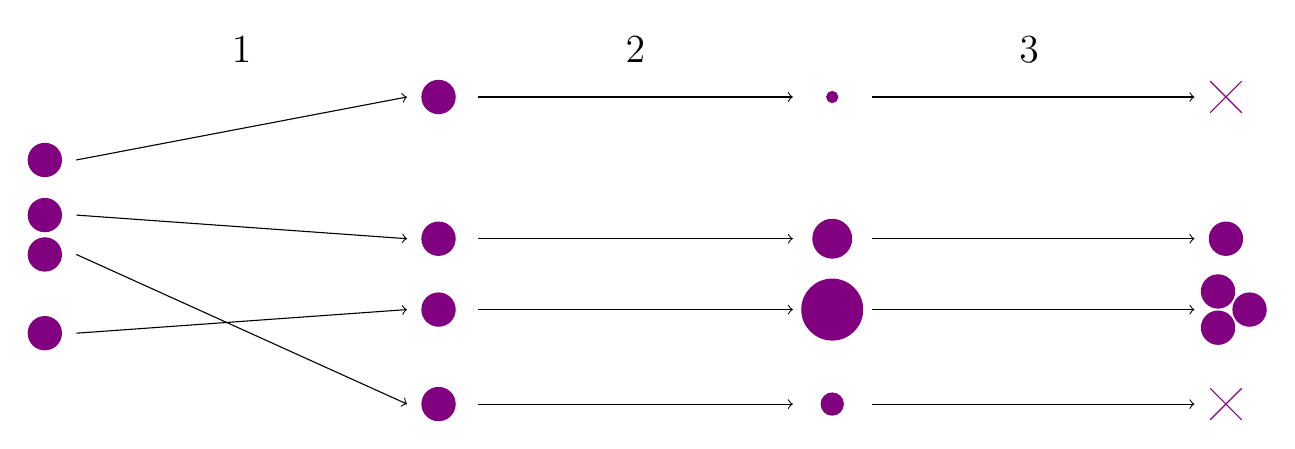
\begin{tikzpicture}
\filldraw[violet] (0,0) circle (6pt);
\filldraw[violet] (0,1) circle (6pt);
\filldraw[violet] (0,1.5) circle (6pt);
\filldraw[violet] (0,2.2) circle (6pt);

\draw[->] (0.4,2.2) -- (4.6,3);
\draw[->] (0.4,1.5) -- (4.6,1.2);
\draw[->] (0.4,1) -- (4.6,-0.9);
\draw[->] (0.4,0) -- (4.6,0.3);

\filldraw[violet] (5,0.3) circle (6pt);
\filldraw[violet] (5,-0.9) circle (6pt);
\filldraw[violet] (5,1.2) circle (6pt);
\filldraw[violet] (5,3) circle (6pt);

\draw[->] (5.5,3) -- (9.5,3);
\draw[->] (5.5,1.2) -- (9.5,1.2);
\draw[->] (5.5,-0.9) -- (9.5,-0.9);
\draw[->] (5.5,0.3) -- (9.5,0.3);

\filldraw[violet] (10,0.3) circle (11pt);
\filldraw[violet] (10,-0.9) circle (4pt);
\filldraw[violet] (10,1.2) circle (7pt);
\filldraw[violet] (10,3) circle (2pt);

\draw[->] (10.5,1.2) -- (14.6,1.2);
\draw[->] (10.5,0.3) -- (14.6,0.3);
\draw[->] (10.5,-0.9) -- (14.6,-0.9);
\draw[->] (10.5,3) -- (14.6,3);

\filldraw[violet] (15.3,0.3) circle (6pt);
\filldraw[violet] (14.9,0.53) circle (6pt);
\filldraw[violet] (14.9,0.07) circle (6pt);
\filldraw[violet] (15,1.2) circle (6pt);

\draw[violet] (14.8,3.2) -- (15.2, 2.8);
\draw[violet] (14.8,2.8) -- (15.2, 3.2);
\draw[violet] (14.8,-0.7) -- (15.2, -1.1);
\draw[violet] (14.8,-1.1) -- (15.2, -0.7);

\node at (2.5,3.6) {\Large{1}};
\node at (7.5,3.6) {\Large{2}};
\node at (12.5,3.6) {\Large{3}};
\end{tikzpicture}
}

\vspace*{25pt}

Sequential Monte Carlo
induces a genealogical process via resampling
\end{center}
\end{column}
\begin{column}{0.45\paperwidth}

\vspace*{-45pt}

\begin{center}
\resizebox{0.85\textwidth}{!}{%
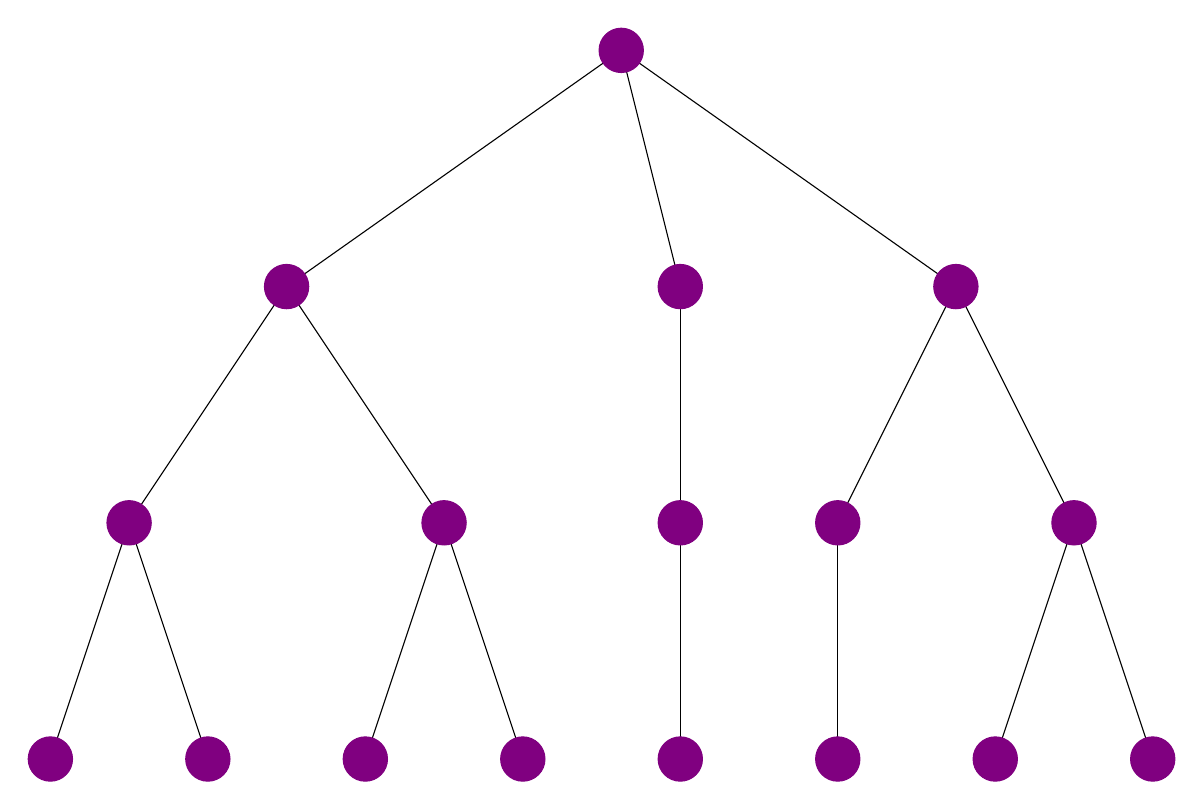
\begin{tikzpicture}
\draw (0,0) -- (1,3);
\draw (2,0) -- (1,3);
\draw (4,0) -- (5,3);
\draw (6,0) -- (5,3);
\draw (8,0) -- (8,3);
\draw (10,0) -- (10,3);
\draw (12,0) -- (13,3);
\draw (14,0) -- (13,3);

\filldraw[violet] (0,0) circle (8pt);
\filldraw[violet] (2,0) circle (8pt);
\filldraw[violet] (4,0) circle (8pt);
\filldraw[violet] (6,0) circle (8pt);
\filldraw[violet] (8,0) circle (8pt);
\filldraw[violet] (10,0) circle (8pt);
\filldraw[violet] (12,0) circle (8pt);
\filldraw[violet] (14,0) circle (8pt);

\draw (1,3) -- (3,6);
\draw (5,3) -- (3,6);
\draw (8,3) -- (8,6);
\draw (10,3) -- (11.5,6);
\draw (13,3) -- (11.5,6);

\filldraw[violet] (1,3) circle (8pt);
\filldraw[violet] (5,3) circle (8pt);
\filldraw[violet] (8,3) circle (8pt);
\filldraw[violet] (10,3) circle (8pt);
\filldraw[violet] (13,3) circle (8pt);

\draw (3,6) -- (7.25,9);
\draw (8,6) -- (7.25,9);
\draw (11.5,6) -- (7.25,9);

\filldraw[violet] (3,6) circle (8pt);
\filldraw[violet] (8,6) circle (8pt);
\filldraw[violet] (11.5,6) circle (8pt);

\filldraw[violet] (7.25,9) circle (8pt);
\end{tikzpicture}
}
\end{center}
What is the limiting process as number of particles $N\to\infty$?
\end{column}
\end{columns}

\vspace*{15pt}

\end{frame}
\end{document}